\subsection*{Q. 3}
\begin{longtable}[c]{ccc|ccc}
\multicolumn{3}{c}{Input\quad} & \multicolumn{3}{|c}{Output\quad} \\ \hline
\endfirsthead
%
\endhead
%
\hline
\endfoot
%
\endlastfoot
%
x       & y       & z      & A       & B       & C      \\ \hline
0       & 0       & 0      & 0       & 1       & 0      \\
0       & 0       & 1      & 0       & 1       & 1      \\
0       & 1       & 0      & 1       & 0       & 0      \\
0       & 1       & 1      & 1       & 0       & 1      \\
1       & 0       & 0      & 0       & 1       & 1      \\
1       & 0       & 1      & 1       & 0       & 0      \\
1       & 1       & 0      & 1       & 0       & 1      \\
1       & 1       & 1      & 1       & 1       & 0      \\ \hline
\end{longtable}

\begin{center}
\begin{karnaugh-map}[4][2][1][$xy$][$z$]
\minterms{1,5,6,3,7}
\implicant{1}{7}
\implicant{7}{6}
\end{karnaugh-map}

\begin{karnaugh-map}[4][2][1][$xy$][$z$]
\minterms{0,4,2,7}
\implicant{0}{4}
\implicantedge{0}{0}{2}{2}
\implicant{7}{7}
\end{karnaugh-map}

\begin{karnaugh-map}[4][2][1][$xy$][$z$]
\minterms{4,3,2,5}
\implicant{4}{5}
\implicant{3}{2}
\end{karnaugh-map}
\end{center}
\vspace{-2em}
\begin{align*}
A&=y+xz\\
B&=x'y'+y'z'+xyz\\
&=(x'+z')y'+(xz)y\\
&=(xz)'y'+(xz)y\\
&=((xz)\oplus y)'\\
C&=xz'+x'z\\
&=x\oplus z
\end{align*}
\centerline{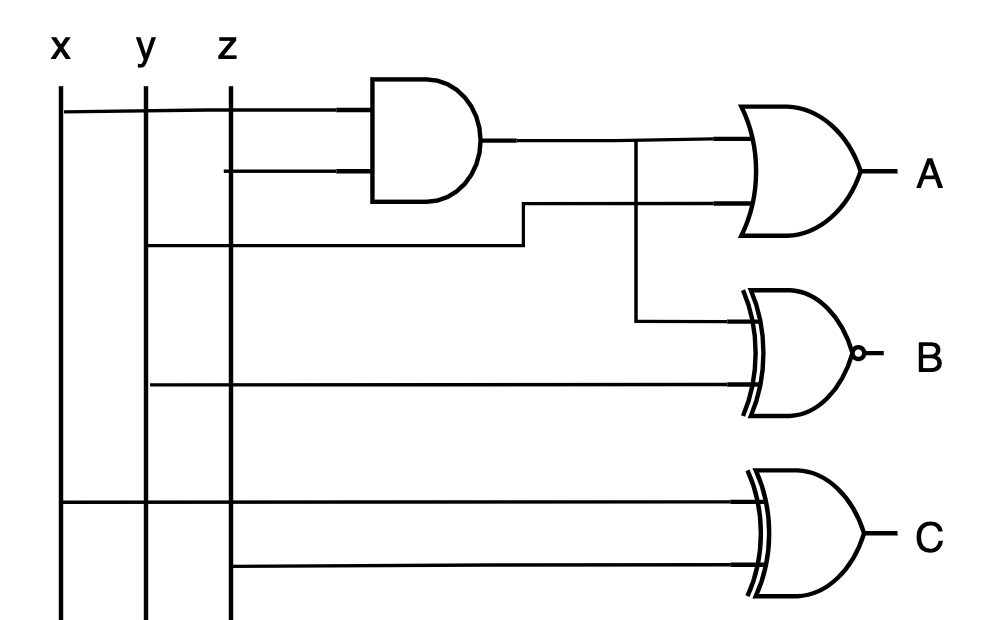
\includegraphics[width=0.4\textwidth]{fig/q3}}
